


\chapter{Waves in Cold Resistive Plasma}
  \label{ch_math}

%ALEX NOTES
%- Why revisit plasma oscillation if it is of little interest?
%- I don't see where Fig 4.1 is referenced in the text. Also it references 5.1?

Before delving into the implementation of the numerical model, it's instructive to consider the fundamental equations of waves in a cold, resistive plasma. 

The evolution of electric and magnetic fields is governed by \amplaw and \farlaw. Notably, the present work takes the linearized versions of \maxeqs; the vectors \vec{E} and \vec{B} indicate perturbations above the zeroth-order magnetic field. 
\begin{align}
  \label{math_maxwells}
  \tensor{\epsilon} \cdot \ddt \vec{E} &= \oomz \curl{B} - \vec{J} & \ddt \vec{B} &= -\curl{E}
\end{align}

Current follows \ohmlaw. For currents perpendicular to the background magnetic field, Kirchhoff's formulation is sufficient. Conductivity is much higher along the magnetic field lines\footnote{The dipole coordinate system is defined rigorously in \cref{sec_coords}; at present, it's sufficient to take \zhat parallel to the zeroth-order magnetic field, and \xhat and \yhat perpendicular to \zhat (and to each other). }, so it's appropriate to also include the electron inertial term\footnote{Electron inertial effects are not included in the model described in \cref{ch_model}, or in the results in \cref{ch_results}; however, their implementation and impact are explored in \cref{ch_inertia}. }. 
\begin{align}
  \label{math_ohms}
  0 &= \tensor{\sigma}_\bot \cdot \vec{E}_\bot - \vec{J}_\bot &
  \frac{1}{\nu} \ddt J_z &= \sz E_z - J_z
\end{align}

Derivatives in \cref{math_maxwells,math_ohms} can be evaluated by performing a Fourier transform. They can then be combined, eliminating the magnetic field and current terms. 
\begin{align}
  \label{disp_setup}
\begin{alignedat}{4}
  & 0 = \vec{E}_\bot && + \frac{\va^2}{\omega^2} \lr{ \vec{k} \times \vec{k} \times \vec{E} }_\bot && + \frac{i}{\ep \omega} \tensor{\sigma}_\bot \cdot && \vec{E}_\bot \\
  & 0 = E_z && + \frac{c^2}{\omega^2} \lr{ \vec{k} \times \vec{k} \times \vec{E} }_z && + \frac{i \op^2 }{\omega \lr{\nu - i \omega} } && E_z
\end{alignedat}
\end{align}

The speed of light, \Alfven speed (including the displacement current correction), plasma frequency, and parallel conductivity are defined in the usual way: 
\begin{align}
  \label{def_basics}
  c^2 & \equiv \frac{1}{\mz \ez} &
  \va^2 & \equiv \frac{1}{\mz \ep} &
  \op^2 & \equiv \frac{n e^2}{\me \ez} &
  \sz & \equiv \frac{n e^2}{\me \nu}
\end{align}

Using the vector identity $\vec{k} \times \vec{k} \times \vec{E} = \vec{k} \, \vec{k} \cdot \vec{E} - k^2 \vec{E}$, \cref{disp_setup} can be reassembled into a single expression, 
\begin{align}
  \label{disp}
  0 &= \lr{ \tensor{ \mathbb{I} } + \frac{1}{\omega^2} \tensor{V}^2 \cdot \vec{k} \, \vec{k} - \frac{k^2}{\omega^2} \tensor{V}^2 + \frac{i}{\omega} \tensor{\Omega} } \cdot \vec{E}
\end{align}

Where $\tensor{ \mathbb{I} }$ is the identity tensor and in \x-\y-\z coordinates, 
\begin{align}
  \tensor{V}^2 &\equiv 
    \mmm{\va^2}{0}{0}
        {0}{\va^2}{0}
        {0}{0}{c^2} &
  & \text{and} &
  \tensor{\Omega} &\equiv 
    \mmm{ \frac{\sp}{\ep} }{ \frac{-\sh}{\ep} }{0}
        { \frac{\sh}{\ep} }{ \frac{\sp}{\ep} }{0}
        {0}{0}{ \frac{\op^2}{\lr{\nu - i \omega}} } 
\end{align}

In \cref{disp}, the expression in parentheses is the dispersion tensor. Nontrivial solutions exist only when its determinant is zero. This gives rise to a seventh-order polynomial in $\omega$, so rather than a direct solution it's necessary to consider limits of specific interest. 

Without loss of generality, the wave vector \vec{k} may be taken to lie in the \x-\z plane --- that is, with $k_y = 0$. The distinction between the two perpendicular directions is discussed in \cref{sec_implications}. 

% -----------------------------------------------------------------------------
% -----------------------------------------------------------------------------
% -----------------------------------------------------------------------------
\section{Guided Propagation}
  \label{sec_par}

The wave vector of a field line resonance aligns closely to the background magnetic field. By supposing that the two align exactly (that is, taking $k_x = 0$), the parallel and perpendicular components  of the dispersion relation are decoupled. 

The parallel-polarized component --- that is, the solution when $E_x = E_y = 0$ --- is quadratic, and thus can be solved directly. 
\begin{align}
  \label{par_par_setup}
  % Parallel propagation, parallel polarization. 
  0 &= \omega^2 + i \nu \omega - \op^2 &
  & \text{so} &
  \omega &= -\frac{i \nu}{2} \pm \sqrt{ \op^2 - \frac{\nu^2}{4} }
\end{align}

It bears noting that the plasma frequency is large --- not just compared to Pc4 frequencies, but even compared to the collision frequencies in the ionosphere\footnote{The collision frequency may match or exceed the plasma frequency for a thin slice at the bottom of the ionosphere, where the density of neutral atoms is large; however, it falls off quickly. Above an altitude of \SI{200}{\km}, conservatively\cite{nicolet_1953}, the plasma frequency exceeds the collision frequency by an order of magnitude or more. }. 

Expanding \cref{par_par_setup} with respect to large \op, the dispersion relation becomes
\begin{align}
  \label{par_par_final}
  % Parallel propagation, parallel polarization. 
  \omega^2 & = \op^2 \pm i \nu \op + ...
\end{align}

\cref{par_par_final} can hardly be called a wave, as it does not depend on the wave vector \vec{k}. Rather, it is the plasma oscillation\footnote{The plasma oscillation is also called the Langmuir wave, after Irving Langmuir. }: electrons vibrating in response to a charge separation along the background magnetic field. 

The plasma oscillation is not specifically relevant to the study of field line resonance. The two phenomena are separated by six orders of magnitude in frequency. The topic is revisited in \cref{ch_inertia} insomuch as it is inseparable from the electron inertial effects in \ohmlaw. 

The perpendicular ($E_z = 0$) components of the dispersion relation give an expression quartic in $\omega$. 
\begin{align}
  \label{par_perp_setup}
  % Parallel propagation, perpendicular polarization. 
  0 &= \omega^4 + 2 i \frac{\sp}{\ep} \omega^3
  - \lr{ 2 k_z^2 \va^2 + \frac{\sp^2 + \sh^2}{\ep^2} } \omega^2
  - 2 i k_z^2 \va^2 \frac{\sp}{\ep} \omega
  + k_z^4 \va^4
\end{align}

Like the parallel-polarized component above, \cref{par_perp_setup} can be solved directly. Noting that $\pm$ and $\opm$ are independent,
\begin{align}
  % Parallel propagation, perpendicular polarization. 
  \omega = \lr{ \frac{\pm \sh - i \sp}{2 \ep} } \opm \sqrt{ k_z^2 \va^2 + \lr{ \frac{\pm \sh - i \sp}{2 \ep} }^2 }
\end{align}

Also like the parallel-polarized component, the exact solution is less useful than its Taylor expansion. The Pedersen and Hall conductivities are large near the ionospheric boundary, but fall off quickly; for the vast majority of the field line, the ratios $\frac{\sp}{\ep}$ and $\frac{\sh}{\ep}$ are small compared to field line resonance frequencies. Expanding with respect to small conductivity gives
\begin{align}
  \label{par_perp_final}
  % Parallel propagation, perpendicular polarization. 
  \omega^2 = k_z^2 \va^2 \opm k_z \va \frac{\sh \pm i \sp}{\ep} + ...
\end{align}

This is the shear \Alfven wave, with a shift to its frequency due to the conductivity of the ionosphere. It travels along the background magnetic field like a bead on a string, with electric and magnetic field perturbations perpendicular to the magnetic field line (and to one another). 

% -----------------------------------------------------------------------------
% -----------------------------------------------------------------------------
% -----------------------------------------------------------------------------
\section{Compressional Propagation}
  \label{sec_perp}

%\todo{Is it fair to say ``compressional'' to mean ``perpendicular'' in terms of propagation? It would be nice to have different jargon for the propagation directions and the polarization directions. }

The partner to guided motion is compressional motion; in order for energy to move across field lines, the wave vector must have a component perpendicular to \zhat. If the wave vector is completely perpendicular to the magnetic field line ($k_z = 0$), the parallel and perpendicular components of the dispersion relation decouple, as in \cref{sec_par}. 

The parallel-polarized ($E_x = E_y = 0$) component of the dispersion relation is
\begin{align}
  \label{perp_par_setup}
  % Perpendicular propagation, parallel polarization. 
  0 &= \omega^3 + i \nu \omega^2
  - \lr{ k_x^2 c^2 + \op^2 } \omega
  - i k_x^2 c^2 \nu
\end{align}

\cref{perp_par_setup} can be solved directly, though its solution (as a cubic) is far too long to be useful. Expanding with respect to the large plasma frequency, gives
\begin{align}
  \label{parallel_math_final}
  % Perpendicular propagation, parallel polarization. 
  \omega^2 & = k^2 c^2 + \op^2 - i \nu \op + ...
\end{align}

This is the O mode, a compressional wave with an electric field perturbation along the background magnetic field. Like the plasma oscillation discussed in \cref{sec_par}, its frequency is very large compared to that of a field line resonance. 

The perpendicular-polarized ($E_z = 0$) component of the compressional dispersion relation is also cubic. 
\begin{align}
  \label{perp_perp_setup}
  % Perpendicular propagation, perpendicular polarization. 
  0 &= \omega^3 + 2 i \frac{\sp}{\ep} \omega^2
  - \lr{ 2 k_x^2 \va^2 + \frac{\sp^2 + \sh^2}{\ep^2} } \omega
   - i k_x^2 \va^2 \frac{\sp}{\ep}
\end{align}

A wave moving across magnetic field lines near the ionospheric boundary will encounter large $\frac{\sp}{\ep}$ and $\frac{\sh}{\ep}$, while at moderate to high altitudes those ratios will be small. Solving \cref{perp_perp_setup} in those two limits respectively gives: 
\begin{align}
  \label{perp_perp_final}
%  \begin{split}
  % Perpendicular propagation, perpendicular polarization. Small conductivity. 
  \omega^2 & = k_x^2 \va^2 \pm i k_x \va \frac{\sp}{\ep} + ... &
  & \text{and} &
  % Perpendicular propagation, perpendicular polarization. Large conductivity. 
  \omega^2 & = k_x^2 \va^2 + \lr{ \frac{\sh \pm i \sp}{\ep} }^2 + ...
%  \end{split}
\end{align}

In both limits, \cref{perp_perp_final} describes a compressional \Alfven wave. The magnetic field perturbation is along the background magnetic field --- indicating compression of the frozen-in plasma --- while the electric field perturbation is perpendicular to both the magnetic field and the wave vector. 

\todo{Double check terminology. Jesse's dissertation disagrees with Bob's notes. }

% -----------------------------------------------------------------------------
% -----------------------------------------------------------------------------
% -----------------------------------------------------------------------------
\section{High Altitude Limit}
  \label{sec_high_alt}

In the limit of large radial distance, it's reasonable to take the collision frequency to zero; doing so also neglects the Pedersen and Hall conductivities. 

Whereas in \cref{sec_par,sec_perp} it was the parallel-polarized component of the dispersion relation that factored out from the other two, the high altitude limit decouples the component polarized out of the \x-\z plane. The \y-polarized dispersion ($E_x = E_z = 0$) is simply:
\begin{align}
  \label{high_y}
  \omega^2 & = k^2 \va^2
\end{align}

\cref{high_y} describes an \Alfven wave with an arbitrary angle of propagation. Depending on the angle between the wave vector and the background magnetic field, it could be guided, compressional, or somewhere in between. Regardless of propagation angle, the electric field perturbation is perpendicular to both the direction of propagation and the magnetic field perturbation. 

The other two components (from $E_y = 0$) of the high altitude dispersion tensor give an expression quadratic in $\omega^2$:
\begin{align}
  \label{high_setup}
  0 &= \omega^4 
  - \lr{ k_x^2 c^2 + k_z^2 \va^2 + \op^2 } \omega^2
  + k_z^2 \va^2 \op^2
\end{align}

Which can be solved for
\begin{align}
  \omega^2 & = \frac{1}{2} \lr{ k_x^2 c^2 + k_z^2 \va^2 + \op^2 }
  \pm \sqrt{ \frac{1}{4} \lr{ k_x^2 c^2 + k_z^2 \va^2 + \op^2 }^2 
    - k_z^2 \va^2 \op^2 }
\end{align}

Noting again that $\op$ is very large, the two roots can be expanded to
\begin{align}
  \label{high_final}
  \omega^2 & = k_z^2 \va^2 \, \lr{ 1 + \frac{ k_x^2 c^2 + k_z^2 \va^2 }{\op^2} }+ ... &
  & \text{and} & 
  \omega^2 & = k_x^2 c^2 + k_z^2 \va^2 + \op^2 + ...
\end{align}

The first is a shear \Alfven wave, as in \cref{par_perp_final}. The second oscillates faster than the plasma frequency; like the plasma oscillation in \cref{par_par_final} and the O mode in \cref{parallel_math_final}, it's far outside the Pc4 frequency range. 

% -----------------------------------------------------------------------------
% -----------------------------------------------------------------------------
% -----------------------------------------------------------------------------
\section{Implications to the Present Work}
  \label{sec_implications}

The present section's findings carry three significant implications for the present work. 

First --- with the exception of the plasma oscillation and similar modes, which are revisited in \cref{ch_inertia} --- waves propagate at the \Alfven speed. This, in combination with the grid configuration, will constrain the time step that can be used to model them numerically. The time step must be sufficiently small that information traveling at the \Alfven speed cannot ``skip over'' entire grid cells\footnote{As is the convention, the time step is scaled down from the smallest \Alfven zone crossing time by a Courant factor, typically 0.1, meaning that it takes at least ten time steps to cross a grid cell. }.

Second, the results of the present section allow an estimate of the magnitude of parallel electric field that might be expected from a field line resonance compared to its perpendicular electric field. Between the full dispersion tenfor form in \cref{disp} and the \Alfven wave described by \cref{high_final}, 
\begin{align}
  \left| \frac{E_z}{E_x} \right| &= \frac{ k_x k_z c^2 }{ \omega^2 - k_x^2 c^2 - \op^2 } \sim \frac{k^2 c^2 }{\op^2}
\end{align}

In essence, the relative magnitudes of the parallel and perpendicular electric fields should be in proportion to the square of the relative magnitudes of the electron inertial length (\SIrange{1}{100}{\km}) and the wavelength (\about\SI{e5}{\km}). That is, parallel electric fields should be smaller than the perpendicular electric fields by six or more orders of magnitude. 

Finally, the dispersion relations shown above indicate how the behavior of a field line resonance should behave as the azimuthal modenumber becomes large. 

Whereas the shear \Alfven wave's dispersion relation depends only on the parallel component of the wave vector, the compressional \Alfven wave depends on its magnitude: $\omega^2 = k^2 \va^2$. If the frequency is smaller than $k \va$, the wave will become evanescent. The wave vector's magnitude can be no smaller than its smallest component, however, and the azimuthal component scales with the azimuthal modenumber: $k_y \sim \frac{\azm}{2 \pi r}$. 

\begin{figure}[!htb]
    \centering
    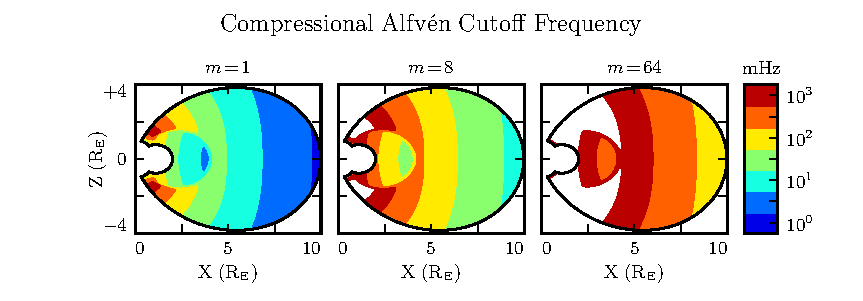
\includegraphics[width=\textwidth]{figures/alfven_cutoff.pdf}
    \caption[Compressional \Alfven Wave Cutoff Frequencies]{
      Taking $k_y \sim \frac{\azm}{2 \pi r}$ as a lower bound for the magnitude of the wave vector, the above figure demonstrates the lowest frequency at which compressional \Alfven waves may propagate as a function of position and \azm. Regions shown in white are off the color scale --- they have a lower bound on the order of \SI{e4}{\mHz} or more. The above \Alfven frequency profile is from Kelley\cite{kelley_1989}, for quiet dayside conditions, as discussed in \cref{sec_profile}. 
    }
    \label{fig_cutoff}
\end{figure}

This imposes a frequency cutoff on compressional \Alfven waves which scales with the azimuthal modenumber, as shown in \cref{fig_cutoff}. At small values of \azm, most of the magnetosphere is conducive to compressional \Alfven waves in the Pc4 frequency range. As \azm increases, and the wave vector with it, the inner magnetosphere becomes increasingly inaccessible to them. 



